\documentclass{standalone}
\usepackage{tikz}
\usepackage{adjustbox}
\usepackage{helvet}  
\usepackage{sansmathfonts}  
\renewcommand{\familydefault}{\sfdefault}  
\usetikzlibrary{arrows.meta,calc,decorations.pathmorphing}
\usetikzlibrary{shapes.geometric, shapes.arrows}
\usepackage[svgnames]{xcolor}


\begin{document}
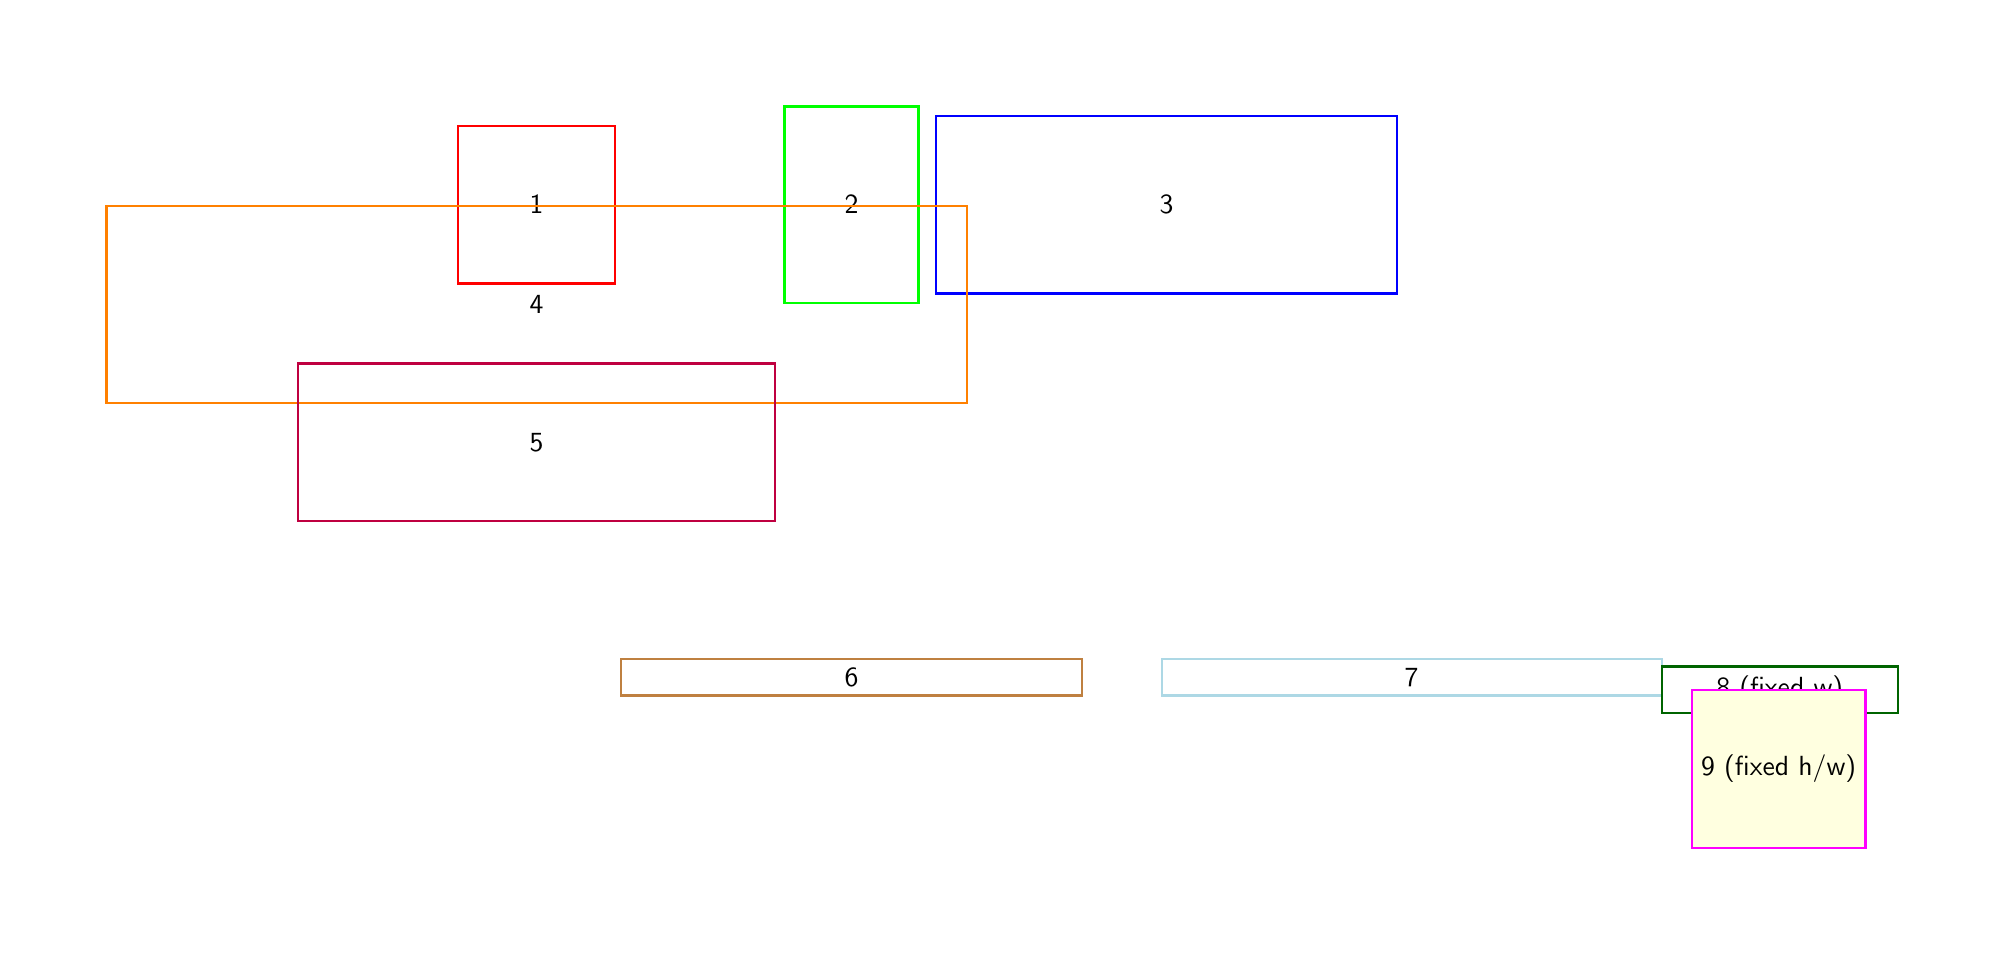
\begin{tikzpicture}
\useasboundingbox (-6.4625,-9.15) rectangle (18.275000000000002,2.25);



\node[minimum width=2cm, minimum height=2cm, shape=rectangle, draw=red, thick] (square1) at (0,0) {\adjustbox{max width=2cm, max height=2cm}{1}};
\node[minimum width=1.7cm, minimum height=2.5cm, shape=rectangle, draw=green, thick] (square2) at (4,0) {\adjustbox{max width=1.7cm, max height=2.5cm}{2}};
\node[minimum width=5.85cm, minimum height=2.25cm, shape=rectangle, draw=blue, thick] (square3) at (8,0) {\adjustbox{max width=5.85cm, max height=2.25cm}{3}};
\node[minimum width=10.925cm, minimum height=2.5cm, shape=rectangle, anchor=north, draw=orange, thick] (square4) at (0,0) {\adjustbox{max width=10.925cm, max height=2.5cm}{4}};
\node[minimum width=6.05cm, minimum height=2cm, shape=rectangle, anchor=north, draw=purple, thick] (square5) at (0,-2) {\adjustbox{max width=6.05cm, max height=2cm}{5}};
\node[minimum width=5.8500000000000005cm, minimum height=0.25cm, shape=rectangle, draw=brown, thick] (square6) at (4,-6) {\adjustbox{max width=5.8500000000000005cm, max height=0.25cm}{6}};
\node[minimum width=6.3500000000000005cm, minimum height=0.3cm, shape=rectangle, anchor=west, draw=LightBlue, thick] (square7) at (7.925000000000001,-6) {\adjustbox{max width=6.3500000000000005cm, max height=0.3cm}{7}};
\node[minimum width=3cm, minimum height=0.3cm, shape=rectangle, anchor=north west, draw=DarkGreen, thick] (square8) at (14.275000000000002,-5.85) {\adjustbox{max width=3cm, max height=0.3cm}{8 (fixed w)}};
\node[minimum width=2cm, minimum height=2cm, shape=rectangle, anchor=north, draw=Magenta, thick, fill=LightYellow] (square9) at (15.775000000000002,-6.15) {\adjustbox{max width=2cm, max height=2cm}{9 (fixed h/w)}};

\end{tikzpicture}
\end{document}